\chapter{Introdução à Teoria de Redes}

A nossa principal ferramenta para modelar o nosso problema surgiu em 1736. Nessa época existia a cidade de Königsberg (atual Kaliningrado), nela passava o Rio Prególia que separava a cidade em 4 partes. Para se caminhar livremente pelas 4 regiões foram construídas 7 pontes que ligavam cada região. Isso gerava uma dúvida intrigante entre os moradores: seria possível sair de uma região e voltar para ela passando por todas pontes apenas uma vez?

Leonhard Euler \cite{Euler1736} se interessou pelo assunto e tentou resolver esse problema. Para isso ele criou uma estrutura chamada Grafo que era composto por pontos (nós) que representavam as regiões e algo ligando entre eles (ligações) que representavam e ignorou toda a forma geométrica de cada um desses objetos. Euler percebeu que para que haja esse caminho é necessário e suficiente que todos os nós tenham um número de ligações pares. Pois para haver uma solução deve existir um caminho de ida e um  de volta para cada vértice, como isso não é verdade para a cidade de Königsberg, então o problema não tem solução.

\begin{figure}[H]
  \centering
  \captionsetup{font=normalsize,skip=1pt,singlelinecheck=on,labelsep=endash}
  \caption{Pontes de Königsberg}
  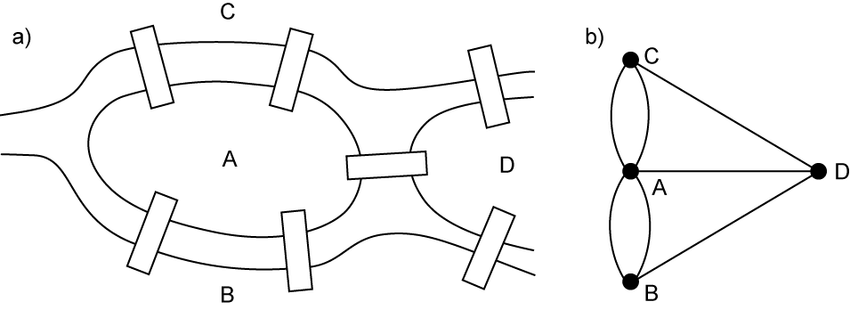
\includegraphics[scale=0.5]{./img/Koenigsberg.png}
  \captionsetup{font=small,position=below,skip=-1pt}
   \caption*{Fonte: Boguslawski, Pawel \cite{Koenigsberg}.}
   \label{Konigsberg}
\end{figure}

A prova de Euler nos mostra que quando queremos modelar algum problema não é necessário considerar todas as variáveis existentes neles, mas o essencial para a solução. Nesse caso o mais importante foi esquematizar o problema usando Grafos e, principalmente, analisar uma estrutura intrínseca ao Grafo.

Com a solução do problema surge a área da matemática chamada Grafos que é a base matemática para o que chamamos em redes. Essa nomenclatura varia de área para área, na física, por exemplo, são sinônimos enquanto que na computação Grafos estão relacionados à problemas de fluxo \cite{Grafos01,Grafos} e Redes são utilizados para problemas visando a estrutura do Grafo e suas interações \cite{network,networks}. Nesse trabalho usaremos os dois como sinônimo.

\section{Conceitos Fundamentais}

Um Grafo $G(\mathpzc{N} ,\mathpzc{L})$ é uma dupla na qual $\mathpzc{N} = \{0,1,2,...,i,...\}$ é um conjunto não vazio de elementos chamados de vértices, ou nós, e $\mathpzc{L}$ é um conjunto não vazio de pares não ordenados de elementos de $\mathpzc{N}$. Dessa forma podemos definir $N = |\mathpzc{N}|$ que mensura a quantidade de vértice que há em $G$ e $L= |\mathpzc{L}|$ que mensura o número de arestas. Essas quantidades também são chamadas de ordem e tamanho \cite{Grafos}, respectivamente, que medem a cardinalidade de $\mathpzc{N}$ e $\mathpzc{L}$.

A partir dessa definição de redes podemos definir a Matriz de Adjacência, ela vai guardar a informação de quem está conectado com quem. Seja uma matriz $A$ quadrada de tamanho $N \times N$, cada elemento da matriz segue a seguinte regra:
\[   
  A_{i,j} = 
     \begin{cases}
       1 \quad \text{se i e j estão conectados}\\
       0 \quad \text{caso contrário.} \\
     \end{cases}
\]

A partir dela surgem características importantes de redes. Se $A_{i,j} = A_{j,i} \forall i,j \in \mathpzc{N}$ então a rede é chamada de não direcionada, se $a_{i,j} \neq a_{j,i} \forall i,j \in \mathpzc{N}$ ela é chamada de direcionada. Isso pode ter diferentes interpretações a depender do contexto inserido. Por exemplo na rede de amigos do Facebook, se o usuário A é amigo de B, então B é amigo de A. No caso do Instagram se A segue B não necessariamente B segue A. No primeiro caso é natural modelarmos utilizando redes não direcionadas, enquanto que no segundo usamos redes direcionadas.

Uma outra forma de guardamos a informação de quem está conectado com quem é a partir da lista de vizinhos. Dois vértices $i$ e $j$ são vizinhos se existe uma ligação entre $i$ e $j$, assim denotamos $\nu(i)$ o conjunto de vizinhos do vértice $i$ para redes não direcionadas. Em redes direcionadas agora temos dois tipos de vizinhos $(i,j)$ e $(k,i)$, portanto denotaremos $\nu_{in}(i)$ todos os vizinhos que têm ligação que chega em $i$ e $\nu_{out}(i)$ todos os vizinhos que têm ligação que sai em $i$.

Por fim, podemos adicionar pesos às nossas ligações, isso têm várias interpretações nos problemas: em uma rede de canos de esgoto, o fluxo que passa em um cano pode ser um peso e em redes de Facebook o nível de amizade pode ser um peso das ligações entre usuários, dentre outros exemplos. Ou podemos adicionar aos vértices como em redes sociais se quisermos estudar a propagação de um vírus a idade ou se ela faz parte de um grupo de risco ou não são parâmetros importantes a serem analisados. Formalmente, um Grafo ponderado $G(\mathpzc{N},\mathpzc{L},\omega)$ é formado por um conjunto de Nós $\mathpzc{N}$, um conjunto de arestas $\mathpzc{L}$ e um mapeamento $\omega: \mathpzc{L}\mapsto \mathbb{R}$ e/ou $\omega: \mathpzc{N}\mapsto \mathbb{R}$. Nesse sentido podemos definir a matrix de pesos $W$ que apresenta uma definição parecida da Matriz de Adjacência, seja $T$ um valor limiar então:

\[   
  w_{i,j} = 
     \begin{cases}
       \omega(i,j) \quad \text{se i e j estão conectados} \\
      0 \quad \text{caso contrário.} \\
     \end{cases}
\]

\begin{figure}[H]
  \centering
  \captionsetup{font=normalsize,skip=0.8pt,singlelinecheck=on,labelsep=endash}
  \caption{Ilustração de Redes e seus Parâmetros}
  \begin{tikzpicture}[make origin horizontal center of bounding box]
    \draw[black, thick] (0,0) -- ($(2,0)+(0,1.5)$);
    \draw[black, thick] (0,0) -- ($(-2,0)+(0,2)$);
    \draw[black, thick] (0,0) -- ($(-2,0)+(0,-1)$);
    \draw[black, thick] (0,0) -- ($(-3.5,0)+(0,-1)$);
    \draw[black, thick] (-3.5,-1) -- ($(-4,0)+(0,1)$);
    \draw[black, thick] (-2,-1) -- ($(-4,0)+(0,1)$);
    \draw[black, thick] (-4,1) -- ($(-2,0)+(0,2)$);
    \draw[black, thick] (-2,-1) -- (-3.5,-1);
    \draw[black, thick] (-4,1) -- (-5.5,0);
    \draw[black, thick] (-3.5,-1) -- (-5.5,0);
    \draw[black, thick] (-4,1) -- (-5.5,-2.5);
    \draw[black, thick] (-3.5,-1) -- (-5.5,-2.5);

    \draw[black, fill=white] ($(0,0) + (0,0)$) circle [radius=0.3] node {0};
    \draw[black, fill=white] ($(2,0) + (0,1.5)$) circle [radius=0.3] node {1};
    \draw[black, fill=white] ($(-2,0) + (0,2)$) circle [radius=0.3] node {5};
    \draw[black, fill=white] ($(-2,0) + (0,-1)$) circle [radius=0.3] node {2};
    \draw[black, fill=white] ($(-4,0) + (0,1)$) circle [radius=0.3] node {4};
    \draw[black, fill=white] ($(-5.5,0) + (0,0)$) circle [radius=0.3] node {6};
    \draw[black, fill=white] ($(-3.5,0) + (0,-1)$) circle [radius=0.3] node {3};
    \draw[black, fill=white] ($(-5.5,0) + (0,-2.5)$) circle [radius=0.3] node {7};
    
    \node at (4,3) {$N = 8$};
    \node at (4,2.5) {$L = 12$};
    \node at (2.5,-1) {$A = $};
    \draw [decorate,
    decoration = {brace}] (3,-3.2) --  (3,1.2);
    \draw [decorate,
    decoration = {brace, mirror}] (7,-3.2) --  (7,1.2);
    \matrix at (5,-1)
  {

    \node {0}; & \node{1}; & \node {1}; & \node {1}; & \node {0}; & \node {1}; & \node {0}; & \node {0};  \\
    
    \node {1}; & \node{0}; & \node {0}; & \node {0}; & \node {0}; & \node {0}; & \node {0}; & \node {0};  \\

    \node {1}; & \node{0}; & \node {0}; & \node {1}; & \node {1}; & \node {0}; & \node {0}; & \node {0};  \\

    \node {1}; & \node{0}; & \node {1}; & \node {0}; & \node {1}; & \node {0}; & \node {1}; & \node {1};  \\

    \node {0}; & \node{0}; & \node {1}; & \node {1}; & \node {0}; & \node {1}; & \node {1}; & \node {1};  \\

    \node {1}; & \node{0}; & \node {0}; & \node {0}; & \node {1}; & \node {0}; & \node {0}; & \node {0};  \\

    \node {0}; & \node{0}; & \node {0}; & \node {1}; & \node {1}; & \node {0}; & \node {0}; & \node {0};  \\
    
    \node {0}; & \node{0}; & \node {0}; & \node {1}; & \node {1}; & \node {0}; & \node {0}; & \node {0};  \\
  };
  \end{tikzpicture}
  \captionsetup{font=small}
  \caption*{Ilustração de uma rede, das suas quantidades de ligações, de nós e da Matriz de Adjacência.\\ Fonte: Elaborado pelo autor}
\end{figure}

\section{Métricas de Redes}

Como discutido anteriormente é muito importante estudarmos a estrutura da rede, pois elas vão governar o comportamento da rede. Para entendermos melhor essa estrutura existem várias métricas \cite{Costa2007} relacionadas à topologia da rede podendo ser classificadas como globais ou locais. As métricas globais são aquelas que estão intrinsecamente ligada ao Grafo, enquanto que as locais estão ligadas à cada vértice da rede.

\subsection{Métricas Globais de Redes}

A primeira delas a ser analisada é a medida de distância entre um vértice e outro. Seja dois vértices $i,j \in \mathpzc{N}$ dizemos que existe um caminho entre $i$ e $j$ se existe uma sequência de vértices $\nu_1,\nu_2,...,\nu_k | (\nu_{s},\nu_{s+1}) \in \mathpzc{L} $ $\forall$ $ 1 \leq s < k $ e $\nu_1 = i,\nu_k = j$. Existem vários caminhos que podem existir entre $i$ e $j$, portanto a nossa distância geodésica entre dois vértices $l_(i,j)$ é definida como a quantidade de arestas do menor caminho entre $i,j$.

Agora que definimos qual é a distância em redes que usaremos, outras métricas surgem a partir dessa definição. Por exemplo temos o menor caminho médio de toda a rede:

\begin{equation}
  \left\langle l \right\rangle  = \sum_{\substack{i,j \\ i\neq j}} \frac{l(i,j)}{N\cdot(N-1)}.
\end{equation}

Esse valor nos dá a informação sobre o quanto em média é necessário caminhar na rede de um nó para outro. Outro valor importante é o chamado diâmetro $d$ que é a maior distância geodésica da rede

\begin{equation}
  d = \max\limits_{i,j \in \mathpzc{N}} l_{i,j}
\end{equation}

Esses valores são bastante importantes para estudos em redes de pequeno mundo \cite{Kleinberg} na qual discutiremos nas próximas sessões.

Uma outra métrica a ser avaliada é quantas conexões cada nó contém. Definiremos o grau $k_i$ do nó $i$ como sendo o número de conexões (ou vizinhos) que o nó $i$ possui para redes não direcionadas. Para redes direcionadas teremos outra divisão entre $k^{in}_i$ e $k^{out}_i$ para os sítios que pertencem a $\nu_{in}(i)$ e $\nu_{out}(i)$. Podemos achar esses valores a partir da Matriz de Adjacência:

\begin{multicols}{2}
  \begin{equation*}
    k^{in}_i = \sum_{j} A_{ij}
  \end{equation*}
  \break
  \begin{equation}
    k^{out}_i = \sum_{j} A_{ji}.
  \end{equation}
\end{multicols}

Além disso podemos também definir o grau médio $\left\langle k \right\rangle$ da rede esse valor tem bastante importância quantitativa quando queremos trabalhar com distribuições de graus.

\begin{equation}
  \left\langle k \right\rangle = \sum_{i \in G}\frac{k_i}{N} = 2\frac{L}{N}
  \label{grau_tamanho}
\end{equation}

Outras duas métricas importantes são a densidade $\rho(G)$ e a reciprocidade $rc(G)$. A primeira mede a razão entre a quantidade de arestas dentro do grafo $G$ pela quantidade total de arestas que o grafo pode suportar. Já a segunda nos apresenta a fração de arestas que existem em ambas as direções, no caso trivial de redes não direcionadas esse valor é igual a 1.

\[   
  \rho(G) = 
     \begin{cases}
      \frac{2L}{N\cdot(N-1)} \quad \text{se a rede for não direcionada, ou }\\
      \frac{L}{N\cdot(N-1)} \quad \text{se a rede for direcionada.} \\
     \end{cases}
\]

\begin{equation}
  rc(G) = \frac{\sum_{i,j} A_{i,j}A_{j,i}}{\sum_{i,j} A_{i,j}}
\end{equation}

Por fim temos uma métrica para analisar o Agrupamento de uma Rede, ou seja quanto que os vértices estão unidos. Essa métrica será definida a partir da probabilidade de um vizinho do nó $i$ estar conectado com outro vizinho de $i$. Existe a definição desse valor a partir da Matriz de Adjacência pela \ref{clustering1}, porém é mais compreensível compreensível pela \ref{clustering2}

\begin{equation}
  C(G) = \frac{\sum_{(i,j,k): i\neq j \neq k}A(i,j)A(j,k)A(k,j)}{\sum_{(i,j,k): i\neq j \neq k}A(i,j)A(j,k)},
  \label{clustering1}
\end{equation}

\begin{equation}
  C(G) = 3\frac{\#Triangulos}{\#Triades}.
  \label{clustering2}
\end{equation}

Em que $\#$ significa número de alguma coisa, no caso estamos contanto o número de triângulos e o número de tríades que aparecem na rede. Essa é a definição do que chamamos de Agrupamento Global, podemos também definir o Agrupamento Local \ref{clusteringlocal} e pro ele o Agrupamento Médio \ref{clusteringmedio}. 

\begin{equation}
  C(i) = 2\frac{\#Triangulos(i)}{\#Triades(i)}.
  \label{clusteringlocal}
\end{equation}

\begin{equation}
  \langle C \rangle = \frac{\sum\limits_{i} C(i)}{N}
  \label{clusteringmedio}
\end{equation}

\begin{figure}[H]
  \centering
  \captionsetup{font=normalsize,skip=0.8pt,singlelinecheck=on,labelsep=endash}
  \caption{Ilustração de Redes e suas Métricas Globais}
  \begin{tikzpicture}[make origin horizontal center of bounding box]
    \draw[black, thick] (0,0) -- ($(2,0)+(0,1.5)$);
    \draw[black, thick] (0,0) -- ($(-2,0)+(0,2)$);
    \draw[black, thick] (0,0) -- ($(-2,0)+(0,-1)$);
    \draw[black, thick] (0,0) -- ($(-3.5,0)+(0,-1)$);
    \draw[black, thick] (-3.5,-1) -- ($(-4,0)+(0,1)$);
    \draw[black, thick] (-2,-1) -- ($(-4,0)+(0,1)$);
    \draw[black, thick] (-4,1) -- ($(-2,0)+(0,2)$);
    \draw[black, thick] (-2,-1) -- (-3.5,-1);
    \draw[black, thick] (-4,1) -- (-5.5,0);
    \draw[black, thick] (-3.5,-1) -- (-5.5,0);
    \draw[black, thick] (-4,1) -- (-5.5,-2.5);
    \draw[black, thick] (-3.5,-1) -- (-5.5,-2.5);

    \draw[black, fill=white] ($(0,0) + (0,0)$) circle [radius=0.3] node {0};
    \draw[black, fill=white] ($(2,0) + (0,1.5)$) circle [radius=0.3] node {1};
    \draw[black, fill=white] ($(-2,0) + (0,2)$) circle [radius=0.3] node {5};
    \draw[black, fill=white] ($(-2,0) + (0,-1)$) circle [radius=0.3] node {2};
    \draw[black, fill=white] ($(-4,0) + (0,1)$) circle [radius=0.3] node {4};
    \draw[black, fill=white] ($(-5.5,0) + (0,0)$) circle [radius=0.3] node {6};
    \draw[black, fill=white] ($(-3.5,0) + (0,-1)$) circle [radius=0.3] node {3};
    \draw[black, fill=white] ($(-5.5,0) + (0,-2.5)$) circle [radius=0.3] node {7};
    
    \node at (4,1.25) {$\langle l \rangle = 1.67$};
    \node at (4,0.75) {$d = 3$};
    \node at (4,0.25) {$\langle k \rangle = 2.035$};
    \node at (4,-0.25) {$\rho = 12/56$};
    \node at (4,-0.75) {$C = 0.375$};
    \node at (4,-1.25) {$ \langle C \rangle = 0.4416$};
  \end{tikzpicture}
  \captionsetup{font=small}
  \caption*{Ilustração de uma rede e sua respectivas Métricas Globais: menor caminho médio, diâmetro, grau médio, densidade, Agrupamento, Agrupamento Médio.\\ Fonte: Elaborado pelo autor}
\end{figure}

\subsection{Métricas de Centralidade}

Ao estudar redes estamos interessados em entender suas estruturas e propriedades, isso já é possível dadas as métricas que apresentamos anteriormente. Contudo, essas métricas globais nos trazem informações sobre a rede como um todo e as propriedades que ela apresenta podem estar diluídas na rede como um todo ou concentrada em sítios específicos. Portanto estudar os sítios em si e a sua importância perante a rede é necessário, para isso usaremos as chamadas Métricas de Centralidade.

Centralidade nesse contexto está ligado à importância, quando falamos de Métricas de Centralidade queremos estudar a importância topológica de cada nó perante a rede. Mas em que sentido seria essa importância? Depende do problema, talvez seja necessário estudar qual o autor mais importante em uma rede de citações de artigos ou qual pessoa devemos retirar de uma rede social para inibir a propagação de \textit{fake-news} para ambas existe uma métrica apropriada para atingir tais objetivos.

A primeira métrica a ser avaliada é propriamente o número de conexões de cada sítio, o grau $k_i$. Ao avaliarmos essa métrica consideramos o sítio central aquele que tem o maior $k_i$, ou seja estamos atrás daquele sítio que apresenta mais ligações.

A segunda métrica importante é a Centralidade de Excentricidade (CE). Excentricidade está definido no dicionário como "desvio ou distância para o centro", no nosso caso a CE vai apontar qual sítio é mais central baseado na maior distância que o sítio pode percorrer na rede, sendo ele o mais central aquele que tem a menor distância máxima. Formalmente $CE(i) \forall i \in \mathpzc{N}$ é definida como:

\begin{equation}
  CE(i) = \frac{1}{\max\limits_{\forall j \in \mathpzc{N}} l_{i,j}}
\end{equation}

Nessa mesma ideia podemos avaliar outras duas métricas parecidas: Centralidade de Proximidade (CP) e Centralidade Harmônica (CH). Em ambas estamos interessados a entender qual é o nó mais central a partir de quanto ele dista dos outros, a diferença entre as duas é que a primeira é calculado pelo inverso da média aritmética e a segunda com a média harmônica.

\begin{equation}
  CP(i) = \frac{N - 1}{\sum_{j \neq i} l_{i,j}}
\end{equation}

\begin{equation}
  CH(i) = \frac{1}{N - 1}\sum_{j \neq i}\frac{1}{l_{i,j}}
\end{equation}

Uma generalização da CP é a Centralidade de média-$p$ ($C_p$), a ideia desta medida de centralidade é usar a noção de média
generalizada das distâncias. Ela é definida como:

\begin{equation}
  C_p(i) = 
  \begin{cases}
    \biggl(\frac{\sum\limits_{j \neq i \in \mathpzc{N}} l(i,j)^p}{N - 1}\biggl)^{-\frac{1}{p}} &\text{se $p \neq 0$}\\
    (\prod\limits_{j \neq i \in \mathpzc{N}} l(i,j))^{-\frac{1}{N - 1}} &\text{se p = 0}
  \end{cases}
\end{equation}

Entretanto a importância de um nó não está associado somente a sua distância entre os outros nós da rede, existem aqueles que são importantes por manterem conexões entre nós. Por exemplo, seja a rede mundial aeroportos que seja construída a partir de nós como sendo os aeroportos e as ligações sendo as viagens entre aeroportos. Nessa situação, imagine que tenha um país altamente conectado entre si, contudo ele só tem um aeroporto que liga esse país ao exterior, esse nó é importante não pela distância dele para os outros aeroportos mas porque ele é o principal e único intermédio entre exterior e o país.

Para ser possível detectar e mensurar esse tipo de importância, considere $\mathbb{L}_{u,v}$ o número de mínimos caminhos que vão de $u$ para $v$ e $\mathbb{L}^{i}_{u,v}$ o número de mínimos caminhos que vão de $u$ para $v$ e passam pelo vértice $i$. Portanto, podemos definir a Centralidade de Intermediação ($CI$) como

\begin{equation}
  CI(i) = \frac{1}{(N - 1)(N - 2)} \sum\limits_{u \neq k} \frac{\mathbb{L}^{i}_{u,v}}{\mathbb{L}_{u,v}}
\end{equation}

% k_shell

% Centralidade de Autovetor

Ao lidarmos com uma rede de uma empresa sabemos que o CEO é muito importante para ela, contudo ele tem contato apenas com os chefes de cada região da empresa e esses chefes não precisariam ter contato com o chefe para ter contato entre si. Então onde estaria a informação de que o CEO é o mais importante? A resposta para essa pergunta está no fato de que o CEO têm ligações com pessoas de importância para rede, algo que não é detectado pelas métricas anteriores Definimos a Centralidade de Autovetor ($CA$) como:

\begin{equation}
  CA(i) = \frac{1}{\lambda}\sum_{j}^nA_{i,j}CA(j)
\end{equation}

Na qual $\lambda$ é o maior auto-vetor associado a matriz de Adjacência de Rede.

% Page_rank

Quando analisamos sites e a sua importância é que essa está ligada com quantas vezes eles são citados por outros sites. Para quantificar isso a Google criou o \textit{Page Rank} ($PR$) \cite{PageRank}. As métricas anteriores são definidas em redes tanto direcionadas quanto não direcionadas, contudo esta só tem sentido quando tratamos de redes direcionadas. Podemos então definir o \textit{Page Rank} como:

\begin{equation}
  PR(i) = (1 - \alpha) + \alpha\sum_{j \neq i}\frac{A_{j,i}PR(j)}{k_{out}(j)}
\end{equation}

Na qual $\alpha$ é um parâmetro de amortecimento.

\section{Modelos de Formação de Redes}

Na sessão anterior discutimos sobre as métricas que tentam quantificar a estrutura da rede, nesse sentido dada um grafo $G$ conseguimos extrair as suas propriedades. Contudo, será que seria possível fazer o contrário? Dado uma propriedade conseguimos criar uma Rede que contenha essas propriedades? Portanto, nessa sessão explicaremos os principais modelos utilizados para formarmos redes artificiais.

\subsection{Rede de Erdös-Rényi}

A Rede de Erdös-Rényi, ou rede aleatória, parte do princípio que nossas conexões com outras pessoas são aleatórias. Ao trabalharmos nesse modelo nós temos o conhecimento de quantos sítios e ligações existem

\subsection{Modelo de Configuração}

Diferente do Modelo de Erdös-Rényi podemos encontrar o caso na qual nós sabemos que o nosso grafo tem uma quantidade $N$ de sítios e sabemos qual a sequência de graus $\{k_i\}$ cada sítio $i$ da rede. Para gerar redes assim usamos o chamado Modelo de Configuração (MC). Esse modelo tem uma restrição de que o número de ligações (que pode ser obtido facilmente por \ref{grau_tamanho}) ser um número par. O modelo segue da seguinte forma:

\begin{enumerate}
  \item Criam-se os $N$ vértices da rede;
  \item Cada vértice $i$ recebe $\kappa_i$ ligações a serem criadas;
  \item Escolhemos o vértice $i$ em ordem decrescente de grau da sequência $\{\kappa_i\}$ (isso serve para facilitar a convergência do modelo);
  \item Escolhemos aleatoriamente outro $j$ sítio da rede que não tenha ligação com $i$ e que ainda não tenha criada todas as $\kappa_j$ ligações e criamos a ligação e reduzimos em 1 o valor de $\kappa_i$ e $\kappa_j$;
  \item Repetimos 3 e 4 até colocarmos todas as ligações na rede.
\end{enumerate}

\begin{algorithm}

  \caption{Modelo de Configuração}\label{alg:MC}
  \begin{algorithmic}
  \Require $k$ \Comment{Essa lista está em ordem decrescente de grau.}
  \Require $edges$\\

  \While{($i \in \mathpzc{N}$) and ($k_i \in k$)} \Comment{Os sítios são escolhidos em ordem decrescente de grau.}
    \State $\kappa_i \gets k_i$
    \While{$j \in \mathpzc{N}$}
      \If{($i \neq j$) and ($k_i \neq 0$)}
          \If{(i,j not in $edges$) and ($k_j \neq 0$)}
            \State $edges$.insert((i,j))
            \State $\kappa_i \gets \kappa_i - 1$
            \State $\kappa_j \gets \kappa_j - 1$
          \EndIf
      \EndIf
    \EndWhile
  \EndWhile
  \end{algorithmic}

\end{algorithm}

\begin{figure}[H]
  \centering
  \captionsetup{font=normalsize,skip=0.8pt,singlelinecheck=on,labelsep=endash}
  \caption{Ilustração do Modelo}
  \begin{tikzpicture}
    \draw[black, thick, dotted] (0,0) -- (-1,-1);
    \draw[black, thick] (0,0) -- (1,1);
    \draw[black, thick, dotted] (0,0) -- (1,-1);
    \draw[black, thick, dotted] (0,0) -- (-1,1);
    \draw[black, fill=white] (0,0) circle [radius=0.25] node {$i$};
    \draw[black, thick, dotted] (1,1) -- (2,2);
    \draw[black, thick] (3,3) -- (2,2);
    \draw[black, thick, dotted] (3,3) -- (4,2);
    \draw[black, thick, dotted] (3,3) -- (2,4);
    \draw[black, fill=white] (3,3) circle [radius=0.25] node {$j$};
  
    \draw[black, thick, dotted] (0,3) -- (0,2);
    \draw[black, thick, dotted] (0,3) -- (0,4);
    \draw[black, thick, dotted] (0,3) -- (-1,3);
    \draw[black, thick, dotted] (0,3) -- (1,3);
    \draw[black, fill=white] (0,3) circle [radius=0.25] node {9};
  
    \draw[black, thick, dotted] (3,0) -- (4,-1);
    \draw[black, thick, dotted] (3,0) -- (2,-1);
    \draw[black, fill=white] (3,0) circle [radius=0.25] node {3};
    
    %\filldraw (0,0) circle (7pt) node[anchor=west, inner sep=0pt]{i};
  \end{tikzpicture}
  \captionsetup{font=small}
  \caption{Funcionamento do Modelo de Configuração, escolhemos dois sítios $i$ e $j$ aleatoriamente e os conectamos. Fonte: Elaborado pelo autor}
  \label{img:MC}
\end{figure}

\section{Modelos de Infecção}

%%%%%%%%%%%%%%%%%%%%%%%%%%%%%%%RECOMENDACAO%%%%%%%%%%%%%%%%%%%%%%%%%%
